\documentclass[12pt]{article}

\usepackage{sbc-template}
\usepackage{graphicx,url}
\usepackage[latin1,utf8]{inputenc}
\usepackage[brazil]{babel}
\usepackage[nonewpage]{imakeidx}
\usepackage[]{float} %Pacote que permite fazer posicionamento específico de figura com parâmetro [H]


\sloppy

\title{Modelagem de interfaces gráficas}

\author{João Victor F. Consonni\inst{1}, Victor H. C. Leite\inst{1}, Mariana D. Souza\inst{1}, \\Matheus Milani\inst{1}, Artur L. Silva\inst{1}, Victor C. Denis\inst{1}, \\Bruno J. M. de Camargo\inst{1}, Danilo B. Cardoso\inst{1}, Lucas K. Kurokawa\inst{1}}

\address{Centro de Matemática, Cognição e Computação\\ Universidade Federal do ABC
  (UFABC)\\
  Av. dos Estados, 5001 - Bangú -- Santo André -- SP -- Brazil
  %\email{jconsonni, victor.costa, dantas.souza, matheus.ferreira, milani.matheus, ,artur.lazarini, v.denis , bruno.camargo, danilo.c@aluno.ufabc.edu.br}
  \email{\{jconsonni, victor.costa,  milani.matheus, }
  \email{artur.lazarini, v.denis, bruno.camargo, danilo.c,}
  \email{dantas.souza, kenzo.kurokawa\}@aluno.ufabc.edu.br}
}

\begin{document} 

\maketitle

\begin{abstract} 
 The software's modeling is one of the main process that shows to the client how the development team understands his requiriments and how to improve them. This document presents some of the screens of the application and which requirimets are in each one.
\end{abstract}

\begin{resumo} 
A modelagem de software é um dos principais processos que mostra ao cliente como o time de desenvolvimento entende os requisitos e como melhora-los. Este documento apresenta algumas telas da aplicação e quais requisitos estão em cada uma.
\end{resumo}

\newpage
\tableofcontents   
\newpage

\section{Introdução}
A popularização dos dispositivos móveis nos séculos XX e XXI, fizeram com que estes equipamentos eletrônicos se tornassem um dos maiores pontos de contato entre os homens e as maquinas. Os GUIs (Graphical User Interfaces), ou interfaces gráficas de usuário, têm se tornado cada vez mais importantes, pois são as interfaces com que os usuários interagem com as funcionalidades do sistema ou aplicativo.

%adicionar um breve texto sobre UX

Estes pontos descritos acima norteiam o conceito de usabilidade, que significam permitir ao usuário utilizar as funcionalidade dos aplicativos de forma fluida, sequencial e em ritmo cadenciado, sem muitos esforços. A utilização destes conceitos propiciam uma melhor experiencia que usuário terá durante o uso do software a ser desenvolvido.  

Diversos padrões podem ser utilizados no desenvolvimento das interfaces gráficas. No estudo de \cite{nielsen1993iterative}, cinco pontos chaves são apresentados para uma aplicação:

\begin{itemize}
    \item \textbf{Fácil de utilizar}, assim o usuário pode rapidamente fazer o aplicativo funcionar sem conhecer o sistema.
    \item \textbf{Eficiente}, possibilitando que o usuário experiente tenha uma alta produtividade com o aplicativo.
    \item \textbf{Fácil de lembrar}, assim usuários não frequentes podem retornar a utilizar o aplicativo após um período de inatividade, sem a necessidade de aprender tudo novamente. 
    \item \textbf{Baixa quantidade de erros}, ou relativamente poucos erros, de modo que o usuário faça poucos erros e que estes erros não sejam catastróficos ao funcionamento do aplicativo.
    \item \textbf{Agradável ao uso}, de modo que usuário possa aproveitar de forma satisfatória o uso do sistema, assim gostando subjetivamente de usar o sistema.
\end{itemize}

Este trabalho tem o intuito de verificar a usabilidade do aplicativo SACI, fornecendo a relação de telas e interfaces, os requisitos do sistema levantados em outros trabalhos e os conceitos apresentados acima.



\section{ Protótipos de interfaces}

Para a prototipação das telas, foi utilizada a plataforma Marvel \cite{marvel2019}, simulando o aplicativo SACI em um sistema Android. Apesar do requisito não funcional [RNF07] do documento de requisitos especificar a utilização de sistemas IOS, não foram desenvolvidas telas especificas para este sistema operacional, dado que a caráter de verificação de usabilidade e cumprimento do documento de requisitos, os protótipos de tela desenvolvidos em Android bastam.

Este documento contem a prototipagem de algumas telas principais do sistema SACI, sendo elas:
\begin{itemize}% talvez colocar a subseção de cada uma das telas
    \item\ref{subsec:Seclogin} - Login de usuário.
    \item \ref{subsec:Seccadastro} - Cadastro de usuário.
    \item \ref{subsec:Secvermapa} - Ver mapa.
    \item \ref{subsec:SeccriaInci} - Criar publicação/incidente.
    \item \ref{subsec:SeceditInci} - Editar publicação/incidente.
    \item \ref{subsec:SecverInci} - Visualizar publicação/incidente.
    \item \ref{subsec:SecMenu} - Expansão menu de navegação.
    \item \ref{subsec:Secnotificacao} - Notificações.
    \item \ref{subsec:Secconfig} - Configurações.
    \item \ref{subsec:SecFaq} - Perguntas frequentes e ajuda.
\end{itemize}

\subsection{Login de usuário}\label{subsec:Seclogin}
A figura \ref{fig:login} representa a prototipação da tela de login do aplicativo e contempla os requisitos: RC21, RC24, TI01, TI02, TI03, TI04 e TI05 contidos no documento de requisitos nas sessões 2.2 e 3.1.1 respectivamente.

A tela foi dividida em três sessões principais sendo elas: formulário de login, links de ação, login com redes sociais.

No formulário de login o usuário do aplicativo deve informar seu login e sua senha, caso queira que suas informações sejam auto preenchidas no próximo login ele deve selecionar a opção lembrar senha, para concluir a ação o usuário deve clicar no botão entrar, caso as informações imputadas estejam corretas o usuário é direcionado a tela principal, caso contrário é informado o erro.

Os links de ação completam a tela de login suportando alguns requisitos do aplicativo permitindo que um usuário novo acesse a tela de cadastro, que um usuário já cadastrado faça login utilizando a biometria ou ainda que um usuário do sistema recupere a senha de acesso.

O espaço de login com redes sociais apresenta os ícones das contas que podem ser utilizadas para realizar login no aplicativo, uma vez autenticado o usuário é direcionado a tela principal do aplicativo.


\begin{figure}[h!]
  \center{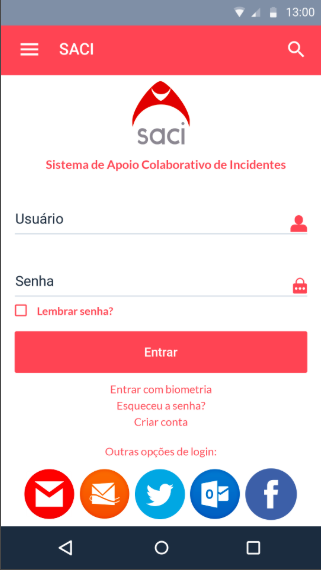
\includegraphics[width=0.5\textwidth]
  {imagens/Interfaces/Login.png}}
  \caption{Login de usuário.}
  \label{fig:login}
\end{figure} 
\vfill%vfill para consertar pagebreak
\pagebreak%Quebra de página para consertar imagens

\subsection{Cadastro de usuário}\label{subsec:Seccadastro}
A figura \ref{fig:newuser} mostra o protótipo elaborado para a tela de cadastro de usuário que contempla os requisitos: RC20, RC23 e TI06 que estão especificados respectivamente nas sessões 2.2 e 3.1.1 do documento de requisitos.

No que se refere a estrutura a tela foi dividida em duas sessões: a primeira sessão apresentando os ícones de redes sociais e a segunda exibindo um formulário de cadastro.

A primeira sessão, como já foi destacado, é utilizada quando o usuário já possui uma conta em algum dos canais apresentados e deseja associar a conta no SACI com sua rede social existente.

Logo abaixo na segunda sessão é apresentada ao usuário uma segunda opção de cadastro onde é requerido informar os dados de e-mail, login, senha e localização residencial sendo esses campos todos obrigatórios para completar o cadastro na aplicação. Caso o formulário esteja completo e o botão criar conta seja pressionado é gerado um novo usuário com as informações especificadas, caso contrário é emitido um pop-up pedindo que usuário finalize o preenchimento das informações antes de prosseguir para a criação da conta.



\begin{figure}[h!]
  \center{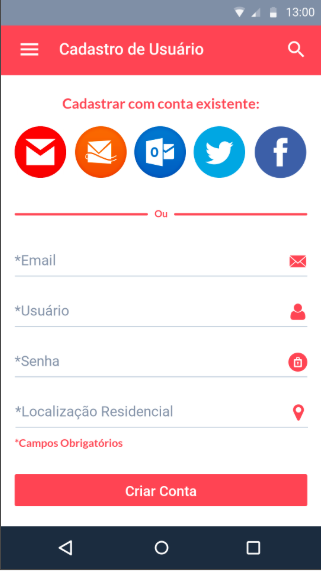
\includegraphics[width=0.5\textwidth]
  {imagens/Interfaces/Cadastro_de_Usuario.png}}
  \caption{Cadastro de um novo usuário.}
  \label{fig:newuser}
\end{figure} 
\vfill%vfill para consertar pagebreak
\pagebreak%Quebra de página para consertar imagens

%Adicionar breve texto de como foi feito, quem fez e quais os requisitos, de acordo com o doc do professor.
\subsection{Ver mapa}\label{subsec:Secvermapa}

Este protótipo foi construído para a tela principal, que é a de visualização do mapa, e atende os requisitos de cliente: RC01 e RC09, e os requisitos funcionais: TP01, TP02, TP03, TP04, TP05, TP06, TP07, TP10 e TP11, que estão especificados respectivamente nas sessões 2.2 e 3.1.2 do documento de requisitos.

A estrutura desta tela é composta de 2 sessões, o mapa e uma barra inferior. 

Na sessão do mapa, é utilizado para que o usuário possa navegar pelo mapa com o toque ou através do campo de busca. Além disso, também é disponibilizado os balões que indicam qual tipo (pela cor), quantas e em quais locais existem publicações sobre incidentes.

Na sessão da barra inferior, o usuário pode utilizar de filtros para fazer uma busca mais avançada de publicações e também é disponibilizado para ele as informações da área em que está ou que ele buscou.



\begin{figure}[h!]
  \center{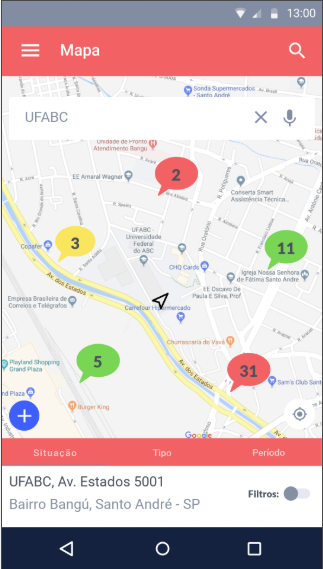
\includegraphics[width=0.5\textwidth]
  {imagens/Interfaces/VerMapa.png}}
  \caption{Ver mapa.}
  \label{fig:vermapa}
\end{figure} 
\vfill%vfill para consertar pagebreak
\pagebreak%Quebra de página para consertar imagens

%Adicionar breve texto de como foi feito, quem fez e quais os requisitos, de acordo com o doc do professor.
\subsection{Criar publicação/incidente}\label{subsec:SeccriaInci}

A \ref{fig:newnot} é a tela de criação de notificação. Nela é possível incluir o tipo de incidente, que ao clicar irá abrir o menu dropdown. Logo abaixo, deverá ser escolhida a localização do incidente, sendo que essa só pode ser feita a 300m do usuário, atendendo ao requisito CI03. 
Além da localização, uma descrição da ação, que é obrigatório como descrito no requisito CI01 poderá ser preenchida no campo cinza.
Logo abaixo, o campo de fotos que mostra as fotos já selecionadas se houverem, um botão para abrir a câmera e outro botão para anexar uma foto já tirada.

Essa tela atende aos requisitos funcionais CI01, CI02, CI03, CI04, CI06 CI07 CI08 e RC02.




\begin{figure}[h!]
  \center{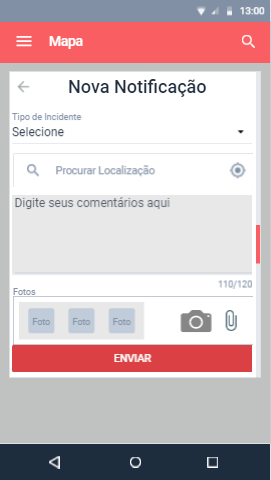
\includegraphics[width=0.5\textwidth]
  {imagens/Interfaces/New_not.PNG}}
  \caption{Criação de nova notificação.}
  \label{fig:newnot}
\end{figure}

\vfill%vfill para consertar pagebreak
\pagebreak%Quebra de página para consertar imagens


%Adicionar breve texto de como foi feito, quem fez e quais os requisitos, de acordo com o doc do professor.
\subsection{Editar Publicação}\label{subsec:SeceditInci}

A figura 3 mostra o protótipo da tela de edição de publicação. Este protótipo contempla os requisitos RC15, RC16, RC19, EI01, EI02, EI03.

Os campos da publicação poderão ser editados livremente caso esta ainda não tenho sido atualizada por outros usuários, caso já tenha, irá seguir o que é definido no documento de requisitos. Para alterar os campos será necessário ao usuário apenas clicar neles, onde irá aparecer as opções de seleção de opção relacionada ao campo ou o input de texto. 

As fotos podem ser removidas selecionando-as nas miniaturas, ao serem selecionadas será exibida a caixa de dialogo para remoção. Para adicionar mais fotos basta clicar no ícone da câmera, que redirecionara o aplicativo para a ferramenta de captura de imagem, ou clicar no ícone de anexo para incluir uma foto que já foi tirada.



\begin{figure}[h!]
  \center{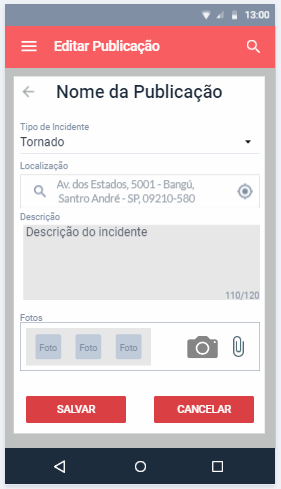
\includegraphics[width=0.5\textwidth]
  {imagens/Interfaces/EditarPub.png}}
  \caption{Editar Publicação.}
  \label{fig:edit_publi}
\end{figure}
\vfill%vfill para consertar pagebreak
\pagebreak%Quebra de página para consertar imagens

%Adicionar breve texto de como foi feito, quem fez e quais os requisitos, de acordo com o doc do professor.

%Adicionar breve texto de como foi feito, quem fez e quais os requisitos, de acordo com o doc do professor.
\subsection{Visualizar Incidente}\label{subsec:SecverInci}
A figura \ref{fig:view_incident} mostra o protótipo da tela de visualização de incidente. Nela, contempla-se todos os requisitos da seção 3.1.6. Visualização de Incidente do documento de requisitos do projeto SACI. 

As primeiras coisas que são notadas ao olhar para a tela de visualização de incidentes são o título da publicação e a foto do incidente. A ideia é que olhando estes dois itens os usuários já tenham noção do que foi o ocorrido. O título não possui um texto padrão já que é o autor da publicação quem o escreve.

Caso o autor queria um detalhe a mais do que foi o causador da situação vista na foto e no título a cor roxa se destaca na tela com letras pequenas de forma a chamar atenção como um item secundário. A ideia da classificação do incidente é identificar o fenômeno gerador.

Para mais detalhes recorre-se à descrição do autor e aos comentários de outros usuários. Também há as opções "Incidente Presente"  e "Incidente Passado" identificando a presença ou continuidade do incidente descrito.


\begin{figure}[h!]
  \center{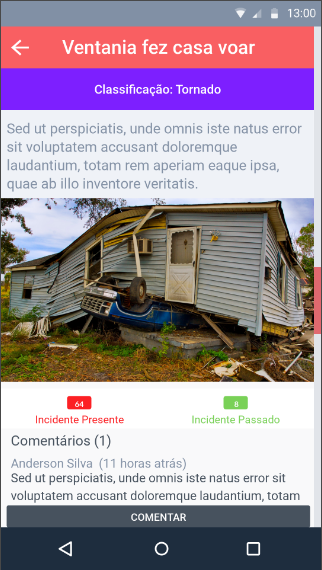
\includegraphics[width=0.5\textwidth]
  {imagens/Interfaces/Visualizacao_Incidente.png}}
  \caption{Visualização de Incidente.}
  \label{fig:view_incident}
\end{figure}
\vfill%vfill para consertar pagebreak
\pagebreak%Quebra de página para consertar imagens

%Adicionar breve texto de como foi feito, quem fez e quais os requisitos, de acordo com o doc do professor.
\subsection{Expansão menu de navegação}\label{subsec:SecMenu}

A figura \ref{fig:view_menulat} demonstra o protótipo elaborado do menu de rápida navegação. Esta tela não contempla diretamente os requisitos do sistema, entretanto esta tela utiliza os conceitos de usabilidade para melhorar a experiencia do usuário, permitindo que haja uma navegação ágil e fácil de todas as outras telas do aplicativo.

Neste menu, o usuário é capaz de transitar entre as funcionalidade a partir de qualquer tela ou ação do aplicativo. Além de visualizar as informações do usuário logado e permitir que o usuário possa se desconectar com o aplicativo, retornando à tela de Login(\ref{subsec:Seclogin}). A seção de perguntas e respostas rápidas (\ref{subsec:SecFaq}) e as configurações gerais da conta logada (\ref{subsec:Secconfig}) podem ser acessados por meio deste menu.

Ao clicar no ícone de menu localizado no canto superior esquerdo das telas, o menu se expandirá. O usuário pode então selecionar qual subseção ou funcionalidade do software ele deseja executar. O ícone de fechar no canto direito do menu faz com que ele retraia e volte a dar foco na tela anterior. Outra maneira de retrair o menu automaticamente é apertar em uma região fora do menu ou apertando no botão voltar do android.



\begin{figure}[h!]
  \center{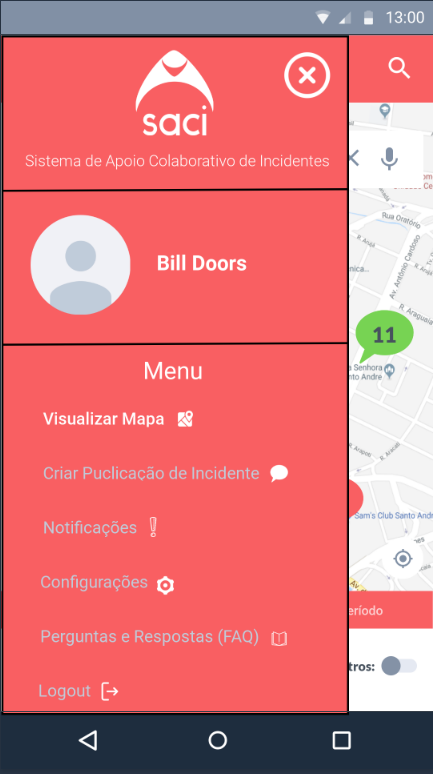
\includegraphics[width=0.5\textwidth]
  {imagens/Interfaces/menu_lateral.png}}
  \caption{Expansão de menu de navegação.}
  \label{fig:view_menulat}
\end{figure}
\vfill%vfill para consertar pagebreak
\pagebreak%Quebra de página para consertar imagens

%Adicionar breve texto de como foi feito, quem fez e quais os requisitos, de acordo com o doc do professor.
\subsection{Notificações}\label{subsec:Secnotificacao}
Em cenários de risco, a Defesa Civil pode emitir alertas para determinadas regiões. Quando isso ocorrer, o sistema do aplicativo verifica a localização do usuário por meio do sistema de geolocalização e, se o usuário estiver próximo à região de alerta ou tiver configurado a região de alerta como favorita, ele recebe uma notificação push-up. Ao clicar na notificação, a tela da Figura \ref{fig:alerta} é exibida.

\begin{figure}[h!]
  \center{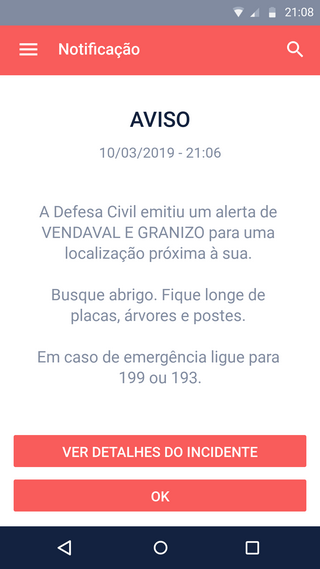
\includegraphics[width=0.5\textwidth]
  {imagens/Interfaces/Alerta.png}}
  \caption{Tela de Notificação de Alertas da Defesa Civil.}
  \label{fig:alerta}
\end{figure}

\vfill%vfill para consertar pagebreak
\pagebreak%Quebra de página para consertar imagens

O texto da mensagem de notificação será adequado ao contexto, informando a data e o horário do alerta, o tipo de incidente, o motivo desta notificação ter sido apresentada ao usuário (proximidade da zona de risco ou região favoritada), assim como breves orientações. Na parte de baixo são exibidos dois botões, permitindo ao usuário ver mais detalhes a respeito do incidente, direcionando-o para a tela de "Visualizar publicação/incidente", ou apenas confirmar o recebimento da mensagem clicando em "OK". 

Essa tela atende aos requisitos RC08, RC10, RC11 e RC12, RNF02, RNF15, RNF16, RNF17, RD01.

%Adicionar breve texto de como foi feito, quem fez e quais os requisitos, de acordo com o doc do professor.
\subsection{Configurações}\label{subsec:Secconfig}
A figura 8 ilustra o protótipo de interface para o a visualização de dados cadastrais, dentro do fluxo de cadastro de um usuário. Pode-se observar os campos de texto com o nome, e-mail e endereço do usuário cadastrados na plataforma de forma clara e objetiva.

\begin{figure}[h!]
  \center{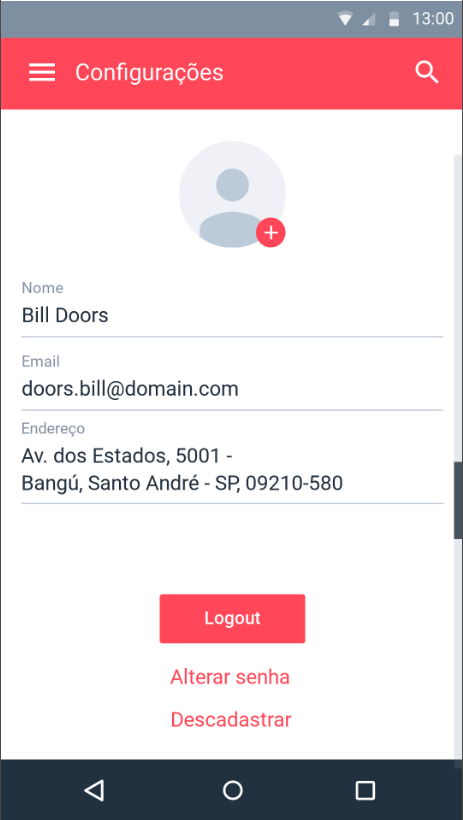
\includegraphics[width=0.5\textwidth]
  {imagens/Interfaces/Configuracoes.png}}
  \caption{Tela de Configurações.}
  \label{fig:configuration}
\end{figure}

Também incluso no fluxo de cadastro de usuários, nesta interface possibilita o usuário alterar sua senha, terminar sua sessão no aplicativo e até excluir sua conta, caso queria.

\vfill%vfill para consertar pagebreak
\pagebreak%Quebra de página para consertar imagens

%Adicionar breve texto de como foi feito, quem fez e quais os requisitos, de acordo com o doc do professor.

\subsection{Perguntas frequentes a ajuda}\label{subsec:SecFaq}
Tela com informações importantes ao usuário, servindo como manual para as principais funções. Pode ser ampliado dependendo das dúvidas do usuário que surgirem pós implementação.

Os requisitos que englobam cada questão podem variar, no detalhe de da figura 10 temos os requisitos do caso de uso "criar uma publicação" (RC02,RC1,CI01, CI02, CI03, CI04, CI05,CI10); "Notificação da defesa civil" (RC08,  RC10,  RC11,  RC12, TP01, TP02, TP03,TP04, TP05, TP06, TP07, TP10 e TP11) e informações sobre o desenvolvimento do projeto. 

\begin{figure}[h!]
  \center{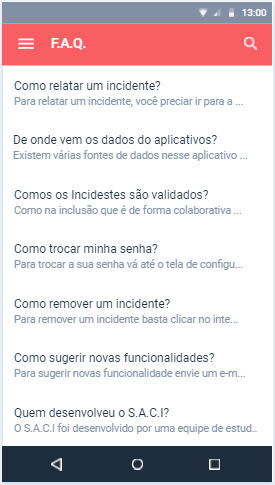
\includegraphics[width=0.5\textwidth]
  {imagens/Interfaces/faq_img.PNG}}
  \caption{Tela de Configurações.}
  \label{fig:Perguntas frequentes e ajuda}
\end{figure}
\vfill%vfill para consertar pagebreak
\pagebreak

\section{Discussão}

Uma boa interface é essencial para um bom produto de software, pois ela é a única responsável pela comunicação dos usuários com o software, ela deve se adequar aos usuários proporcionando uma boa usualidade para o dia a dia. Quanto mais amigável, fácil de utilizar e com componentes mais padronizados, melhor.

Além disso, a modelagem dos protótipos de interface proporcionam um novo ponto de vista sobre o projeto, um ponto de vista bem acessível aos clientes e futuros usuários da aplicação, os protótipos devem ser apresentado aos clientes para validação e confirmação dos requisitos já definidos anteriormente e para possíveis apresentações de melhorias ou modificações. Para se alcançar uma interface de qualidade é essencial uma validação constante com os usuários.

Por fim, as interfaces servem como mais um meio de validação de requisitos e atualização dos mesmos, pois durante o a sua modelagem nos damos conta de muitos fatores e detalhes relevantes a aplicação que podem ser difíceis de serem visualizados sem estes protótipos.


\section{Conclusão}

A possibilidade de definir a identidade visual do software antes do desenvolvimento do front-end permite que decisões de design sejam tomadas muito mais rapidamente e prováveis alterações sejam feitas de forma mais direta e sem grande trabalho. Com a facilidade de ter em mãos a interface gráfica do projeto todo o desenvolvimento fica mais orientado e os desenvolvedores mais alinhados com o que precisa ser desenvolvido.

O desenvolvimento das interfaces gráficas do SACI pela equipe consolidou a ideia do plicativo que tínhamos em nossas mentes com detalhes diferentes para cada integrante do grupo. Devido o documento de requisitos estar bem separado quanto as funcionalidades do software foi fácil a definição dos casos de uso e consequentemente quais as telas necessárias para o funcionamento do SACI.

O grupo não desenvolverá o front-end do aplicativo mas ficou evidente o quão facilitador é definir os detalhes de design, as decisões de posição, cor, tamanho e formas sem precisar desenvolver as linha de código.

\section{Como o processo de Scrum foi seguido pela equipe}
Para este entregável, a equipe SCRUM se organizou de forma a permitir que cada membro do grupo pudesse fazer, ao menos, uma tela da interface. Assim, utilizamos o Trello como ferramenta de distribuição de tarefas e, ao invés de definir na planning o que cada um faria, criamos os cards no Trello e deixamos para cada um escolher uma tela. A divisão de telas ficou como descrito na Tabela \ref{tabela}.

\begin{table}[h!]
\centering
\begin{tabular}{|l|l|}
\hline
\multicolumn{1}{|c|}{\textbf{Tela}} & \multicolumn{1}{c|}{\textbf{Responsável}} \\ \hline
Login de usuário & Mariana D. Souza \\ \hline
Cadastro de usuário & Mariana D. Souza \\ \hline
Ver Mapa & Lucas K. Kurokawa \\ \hline
Criar Publicação & Victor C. Denis \\ \hline
Editar Publicação & Danilo B. Cardoso \\ \hline
Visualizar Incidente & Victor H. C. Leite \\ \hline
Expansão Menu de Navegação & Artur L. Silva \\ \hline
Notificações & João Victor F. Consonni \\ \hline
Configurações & Matheus Milani \\ \hline
Perguntas Frequentes e ajuda & Bruno J. M. de Camargo \\ \hline
\end{tabular}
\caption{Responsável por Tela}
\label{tabela}
\end{table}

Para o desenvolvimento das telas, criamos uma única conta no Marvel, uma ferramenta online de prototipagem de interfaces para aplicativos voltados para smartphones. Compartilhar uma única conta foi essencial para garantir a padronização no estilo das telas, principalmente na utilização da mesma paleta de cores em todas elas.

Apesar de várias das telas já terem sido previamente elaboradas durante o desenvolvimento dos diagramas de casos de uso, aproveitamos este último entregável para revisitar aquelas telas e propor um novo layout, ainda preocupados em contemplar os pontos levantados no documento de requisitos, porém, desta vez, sob a luz dos modelos arquiteturais 4+1 e C4.



A elaboração deste documento teve duas dificuldades principais. A primeira foi a de cada um desenvolver uma tela estando todos remotos e disponíveis em momentos distintos. A segunda, foi recapitular toda a documentação que foi feita até aqui para que as telas refletissem as especificações, diagramas e modelos construídos nos documentos anteriores. Por fim, acredito que fizemos um bom trabalho em atingir os objetivos da sprint, mesmo diante das dificuldades mencionadas. 

\bibliographystyle{sbc}
\bibliography{main}

\end{document}